\begin{figure}
\begin{tabular}{cc}
\begin{subfigure}[b]{0.45\textwidth}
\begin{center}
\begin{allLangEnvFoot}
~{\scriptsize \textcolor{mygray}{   }}~   
~{\scriptsize \textcolor{mygray}{S0:}}~ i32 sum_list (List l) {
~{\scriptsize \textcolor{mygray}{S1:}}~   i32 sum $\coloneqq$ ${\tt 0_{i32}}$;
~{\scriptsize \textcolor{mygray}{S2:}}~   while ${\tt \neg (l\ is\ LNil)}$:
~{\scriptsize \textcolor{mygray}{S3:}}~     // (l is LCons);
~{\scriptsize \textcolor{mygray}{S4:}}~     sum $\coloneqq$ sum + ${\tt l.val}$;
~{\scriptsize \textcolor{mygray}{S5:}}~     l   $\coloneqq$ l.next;
~{\scriptsize \textcolor{mygray}{S6:}}~   return sum;
~{\scriptsize \textcolor{mygray}{SE:}}~ }
\end{allLangEnvFoot}
\end{center}
\caption{\label{fig:llTraverseSpec}(Abstracted) Spec IR}
\end{subfigure}%
&
\begin{subfigure}[b]{0.55\textwidth}
\begin{center}
\begin{allLangEnvFoot}
~{\scriptsize \textcolor{mygray}{\ \ \ }}~ unsigned sum_list (lnode* l);
~{\scriptsize \textcolor{mygray}{C0:}}~ i32 sum_list (i32 l) {
~{\scriptsize \textcolor{mygray}{C1:}}~   i32 sum $\coloneqq$ ${\tt 0_{i32}}$;
~{\scriptsize \textcolor{mygray}{C2:}}~   while ${\tt l \neq 0_{i32}}$:
~{\scriptsize \textcolor{mygray}{C3:}}~     sum $\coloneqq$ sum + $\structPointer{\tt l}{m}{lnode}{val}$;
~{\scriptsize \textcolor{mygray}{C4:}}~     l   $\coloneqq$ $\structPointer{\tt l}{m}{lnode}{next}$;
~{\scriptsize \textcolor{mygray}{C5:}}~   return sum;
~{\scriptsize \textcolor{mygray}{CE:}}~ }
\end{allLangEnvFoot}
\end{center}
\caption{\label{fig:llTraverseC}(Abstracted) C IR}
\end{subfigure}%
\\
\begin{subfigure}[b]{0.45\textwidth}
\begin{center}
{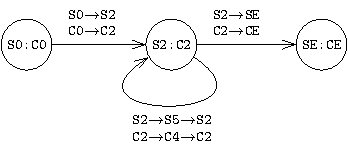
\includegraphics[scale=1.1]{chapters/figures/figSumListProductCfg.pdf}}
\end{center}
\caption{\label{fig:llTraverseProduct}Product-CFG}
\end{subfigure}%
&
\begin{subfigure}[b]{0.55\textwidth}
\begin{center}
\begin{footnotesize}
\begin{tabular}{|c|l|}
\hline
\tt PC-Pair & \multicolumn{1}{c|} {\tt Invariants} \\
\hline
\hline
${\tt (S0:C0)}$ &
\Tstrut ${\tt {\circled{P}}\  l_{S}\indEq{}Clist^{lnode}_{m}(l_{C})}$ \\
\multirow{2}{*}{${\tt (S2:C2)}$} &
\Tstrut \Bstrut ${\tt {\scriptsize \circled{I1}}\  l_{S}\indEq{}Clist^{lnode}_{m}(l_{C})}$ \\ & ${\tt {\scriptsize \circled{I2}}\  sum_{S}=sum_{C}}$ \\
${\tt (SE:CE)}$ &
\Tstrut \Bstrut ${\tt {\circled{E}}\  ret_{S}=ret_{C}}$ \\
\hline
\end{tabular}
\end{footnotesize}
\vspace{13px}
\end{center}
\caption{\label{fig:llTraverseProductInv}Node Invariants of the Product-CFG}
\end{subfigure}%
\\
\end{tabular}
\caption{\label{fig:llTraverseSpecAndC}Spec and C programs for traversing a linked list. \Cref{fig:llTraverseProduct} shows the Product-CFG between the IRs in \cref{fig:llTraverseSpec,fig:llTraverseC}. The inductive invariants of the Product-CFG are given in \cref{fig:llTraverseProductInv}.}
\end{figure}
